%!TEX root = ../main.tex

\documentclass[../main.tex]{subfiles}

\begin{document}

\chapter{Background}
\label{chapter:background}

This chapter reviews some of the concepts required to understand the proposed solution in this thesis. This chapter is organized as follows. Section~ reviews some aspects of geometry related to polygons, Section~ reviews representation of robot dynamics. 

\section{Robot Dynamics}
\label{section:background_robot_dynamics}

Throughout the thesis, we make multiple references to the coverage workspace of a robot. The coverage workspace refers to the region in the environment, such as a room in a house, that is required to be covered. The workspace is denoted by $W\subset\mathbb{R}^2$. For the purpose of this thesis, we assume that $W$ is connected. An example of a workspace is demonstrated in Figure~\ref{fig:workspace_and_system}.

\begin{figure}
	\centering
	\subfile{img/chapter_3/workspace_and_system}
	\caption{The workspace polygon and a point model of the robot.}
	\label{fig:workspace_and_system}
\end{figure}

%Since our assumption for the workspace is only that it is connected, the workspace may contain $k$ obstacles. These obstacles are denoted by $O_1,\ldots,O_k$. The obstacles are subsets of $W$ are subregions contained entirely in the workspace that are not reachable by the robot. 


%\begin{definition}[Free Workspace]
%A free workspace is defined as a subset of $W$ that is free of obstacles:
%	\begin{equation}
%		W_{\text{free}}=W\setminus(O_1\cup\dots O_n).
%	\end{equation}
%\end{definition}

The robot that is to be used for coverage has some dynamics. These dynamics give rise to the configuration space of a robot. The configuration space is denoted by $Q$. For the purposes of this work, the configuration space can be thought of as a plane in $\mathbb{R}^2$. In the path planning works, an important subset of the configuration space is the free configuration space. That is, $Q_{\text{free}}\subseteq Q$ is a configuration space of a robot that is free from any collisions. Figure~\ref{fig:configuration_space} demonstrates the free configuration space for a point robot with a circular base. It is important to note that some areas are not accessible such as the corners of the workspace. Hence, these areas are not in the free configuration space since if a robot would attempt to reach these points, it would collide with the workspace boundary. Therefore, a feasible path is called a continuous path that is entirely in the free configuration space:
\begin{equation}
	p=\bigcup q_i, q_i\in Q_{\text{free}}.
\end{equation}
A set of all feasible paths is denoted by $P$:
\begin{equation}
	P=\{p_i\ |\ p_i\subseteq Q_{\text{free}}\}.
\end{equation}

\begin{figure}
	\centering
	\subfile{img/chapter_3/configuration_space}
	\caption{An example of a free configuration space shown in orange for a point robot.}
	\label{fig:configuration_space}
\end{figure}

As an example, in this thesis, a kinematic model of Dubins' car~\cite{dubins1957curves}is used. The kinematic model is shown as follows:
\begin{equation}
	\begin{aligned}
		& \dot{x}=V\cos{\theta}\\
		& \dot{y}=V\sin{\theta}\\
		& \dot{\theta}=u.
	\end{aligned}
\end{equation}
where $(x,y)$ is a position of the robot and $V$ is the linear constant speed of the car, $u$ is the turn rate, which is bounded. The maximum turning rate corresponds to the minimum  turning radius, often refeered to as $r$ in this thesis. In this case, the configuration space of the car is $R^2\times\Theta$

We now shift our focus to the paths that these robots traverse. Throughout the thesis, we make numerous references to straight line segments and transition segments. Straight line segments are paths that consists of a straight line. In other words, a robot traversing a straight line segments will never change its heading. This means that a straight line segment only has a linear component. On the other hand, a transition segment is a path where the robot does change its heading. In other words, the angular component of such a path is non zero.

Any coverage robot is equipped with a coverage tool. When this tool is operational, there is an associated coverage footprint with it. The location of this footprint and the exact region covered by this footprint depend on the physical location of this footprint in the robot. To formalize this relation, a function is introduced called the coverage map, $\mathcal{M}:Q\to \mathbb{R}^2$. The coverage map function maps the configuration $q$ of a robot to a set of points in $\mathbb{R}^2$ that are located under the footprint. Since the location of the coverage footprint is determined by the configuration of the robot, it is naturally to ask what areas can be covered given the free configuration space. A set of points that can be covered given a free configuration space is called the coverable space and is denoted by $\mathbb{C}$. An example of a coverable space determined by the configuration space for a disk robot is shown in Figure~\ref{fig:coverable_space}. Formally, the coverage space is defined as follows:
\begin{equation}
	\mathbb{C}=\bigcup_{q\in Q_{\text{free}}}\mathcal{M}(q).
\end{equation}
\begin{figure}
	\centering
	\subfile{img/chapter_3/coverable_space}
	\caption{An example of a coverable space.}
	\label{fig:coverable_space}
\end{figure}






%\begin{definition}[Robot Location Map]
%\label{definition:location_map}
%Given a robot with dynamics, the configuration space of the robot is $Q$. A location map $\mathcal{L}:Q\to W$ is a function mapping the configuration $q\in Q$ of the robot to a \emph{center} point of the robot. For example, in Figure~\ref{fig:configuration_space}, the location of the center of the robot is $(x,y)$.
%\end{definition}


%\begin{definition}[Free Configuration Space]
%\label{definition:free_c_space}
%The free configuration space is defined as:
%	\begin{equation}
%	\begin{aligned}
%		Q_{\text{free}}=\{q\in Q\ |\ \mathcal{B}(q)\ \text{is inside}\ W_{\text{free}}\}.
%	\end{aligned}
%	\end{equation}
%\end{definition}


%\begin{definition}[Path Metric]
%A path metric is a function $\mathcal{E}:P\to\mathbb{R}$ that assign a cost to a feasible path. This cost is usually determined by the application.
%\end{definition}


\section{Geometric Preliminaries}
\label{section:background_geometry}

In this section, a review of some of the concepts in geometry is reviewed.

A \emph{simple polygon} is a non-intersecting chain of straight line segments forming a closed loop and specified as a set of points, i.e., $Z=\{v_i\in\mathbb{R}^2|i=1,\ldots,n\}$. Note that since the chain is a circuit, any $v_i\in Z$ has two adjacent line segments. A \emph{boundary of a simple polygon} is a set of points, $\partial Z$, along a line connecting any two adjacent vertices of a chain. A \emph{clockwise simple polygon} is a simple polygon where vertices are specified in a clockwise order. We associate these types of simple polygons with holes in the workspace. A \emph{counter-clockwise simple polygon} is a simple polygon where vertices are specified in a counter-clockwise order. This type of simple polygons are associated with the external boundary of the workspace. Finally, a \emph{polygon} is a set of clockwise and counter-clockwise simple polygons. For clarity, we will refer to simple polygons as chains and reserve the term polygon for a set of chains, i.e., $P=\{Z_0,\ldots,Z_m\}$. $Z_0$ is a counter-clockwise chain (i.e., the boundary) and all subsequent $Z_i$ are clockwise chains (i.e., holes). A \emph{boundary of a polygon} is the set of points defined as $\partial P=\bigcup^M_{i=1}\partial Z_i$ where $Z_i\in P$.

A \emph{reflex vertex} is a vertex in one of the chains of $P$ that has an internal angle of more than $\pi$. As such, a polygon is \emph{convex} if and only if there are no reflex vertices. Conversely, a polygon is non-convex if and only if it contains at least one reflex vertex. Note that the presence of a hole guarantees at least one reflex vertex.

\section{Traveling Salesman Problem Preliminaries}
\label{section:GTSP}

In this section, we review one of the famous problems in computer science called the Travelling Salesman Problem. The formulation of the problem is introduced. WE then move on to the generalization of TSP called Generalized TRavelling Saelsman Problem.

First we go over the inputs to the problem. The TSP is defined over a complete graph $G=(V,E,w)$. $V$ is a set of vertices in the graph. $E$ is a set of edges in the graph. Since $G$ is complete, there exists an edge between any pair of verticies in $V$. Every edge $e\in E$ has an associated weight $w$ in it. An example of a graph is shown in Figure~\ref{fig:complete_graph}. Here, the vertices are shown as yellow nodes. The edges are shown as black lines connecting the dots. Note that every node has a line connecting it to every other node.
\begin{figure}
	\centering
	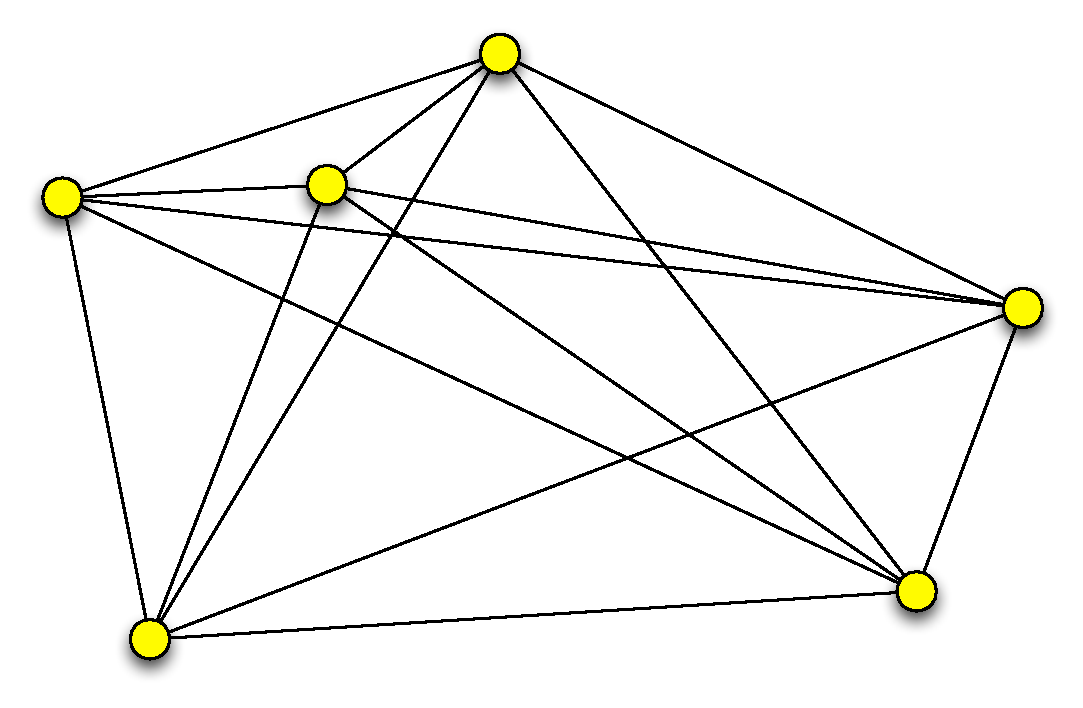
\includegraphics[scale=0.5]{chapter_3/Graph_novehicle.pdf}
	\caption{An example of a complete graph $G$.}
	\label{fig:complete_graph}
\end{figure}


\begin{problem}
Given a complete graph $G=(V,E,w)$, comptue a minimum cost tour of $G$ where every vertex is visisted exactly once.
\end{problem}

This is problem is knonw to be NP-hard. As such, the search space for the solution \emph{blows up} as the combinatrial size of the input. Nevetherless, there are various solutions available that provide approximate and suboptimal solutions with relativly fast compute time. One of these is an algorithm using a Lin-Kernighan TSP heuristic~\cite{helsgaun2009general}. This work makes use of the solver extensivly.

Another side of this problem is a more general form of TSP called the Generalized Travelling Salesman Problem. The inputs to this problem are the same with the exception of the following. A vertex partition $P=\{V1,\ldots,V_{\ell}\}$ is also provided. The vertex partition is a set of subsets of $V$ with no overlapping elements. In other words, 



Suppose a complete graph $G=(V,E,w)$ is given where $V$ is a set of vertices, $E$ is a set of edges, and $w$ is a set of edge weights. Suppose $V$ is partitioned into pairwise disjoint sets $\{V_1,\ldots,V_p\}$ where $V_i\subset V$. The Generalized Traveling Salesman Problem (GTSP) is the problem of computing a tour that visits exactly one vertex from each $V_i$ such that the length of the tour is minimized. The TSP is a special case of the GTSP where $|V_i|=1$ for each $i$ and is NP-hard.

%\section{Contours Introduction}
%\label{section:background_contours}

%In this section, the concept of contours is introduced and some of the related material in medial axis and straight skeletons is reviewed.

%Blum~\cite{blum1967transformation} in 1967 have proposed a notion of medial axis as a shape description. The motivation behind this was generation of ways to represent a shape. The medial axis is defined as follows.
%\begin{definition}
%Suppose a simple polygon $G$ is given then the medial axis $M(G)$ is a set of points $\{q\}$ in the interior of $G$ such that there are at least two points on the object's boundary that are equidistant from $\{q\}$ and are closest to $\{q\}$.
%\end{definition}
%There is an associated radius function that maps every points on $M(G)$ to a radius. This radius specifies the distance of each points on the axis to the boundary. This allows for reconstruction of the original shape by looking at the union of circles centered at each point of $M(G)$ with the corresponding radius. Lee~\cite{lee1982medial} have proposed a $\mathbb{O}(b\log n)$ algorithm for computing medial axis where $n$ is the number of edges.

%Related to medial axis is the concept of straight skeletons introduced by Aichholzer~\cite{aichholzer1996novel}. Because of its structure, it can be misconstrued to be equivalent to medial axis. However, even though, for convex polygons they are identical, the difference arise at the reflex vertices of a polygon. The straight skeleton are defined in terms of a shrinking process where all points on the boundary of a polygon are moving inwards with the same speed. In the process there are two events that can happen. The first event is the edge event. This is where an edge is reduced to zero length in the process of shrinking resulting in its two adjacent edges be adjacent to each other instead. The second event is a split event where the polygon is split into two. Reflex vertices result in this type of event. 
%During the shrinking process, a set of nested polygons is generated. These are of particular interest with respect to this work.

%The straight skeleton is defined as the union of the pieces of angular bisectors traced out by polygon vectices as they are shrinked.
\end{document}